% !TEX root = CI_Adoption.tex

\section{Results and Discussion}
\label{sec:results}
We discuss changes in development practices after CI adoption along four 
dimensions: commit frequency, code churn, pull requests resolution efficiency,
issue tracking, and testing. 

%\subsection{Preliminaries}
%\label{sec:examples}
%
%Before diving into quantitative analysis we eyeballed several projects in our 
%collection. 
%We observed that on several occasions \Tvis has been adopted as part of a 
%larger scale restructuring effort. 
%For instance, \texttt{allendevco/pill-logger} has started using \Tvis on November 
%20, 2013; in the same period developers have changed the project build system 
%from Ant to Gradle and, as a consequence of that, also changed the way the 
%project folders are organized.
%Similarly, \texttt{Netflix/denominator} has introduced \Tvis on March 13, 2015
%after an active development period of daily commits starting on March 3.
%On the very same date \Tvis has been introduced, the project updated library 
%dependencies and restructured tests, while on the next day it added examples 
%and removed support of DiscoveryDNS.
%This rather active development continued until the version 4.5.0 has been 
%released on April 6, 2015.
%The project had three additional commits in April and then went to a recess 
%until early August. 
%Examples such as \texttt{allendevco/pill-logger} and \texttt{Netflix/denominator} 
%suggest that the activity immediately prior and immediately after introduction 
%of \Tvis might not be representative for the project's overall software development
%practices.
%Therefore, to limit the risk of our trends being biased by extraordinary project 
%activity during the transition period, we decided to exclude one month before 
%the first \Tvis build and one month after it, in our quantitative analyses below.



\begin{figure}[t]
\centering
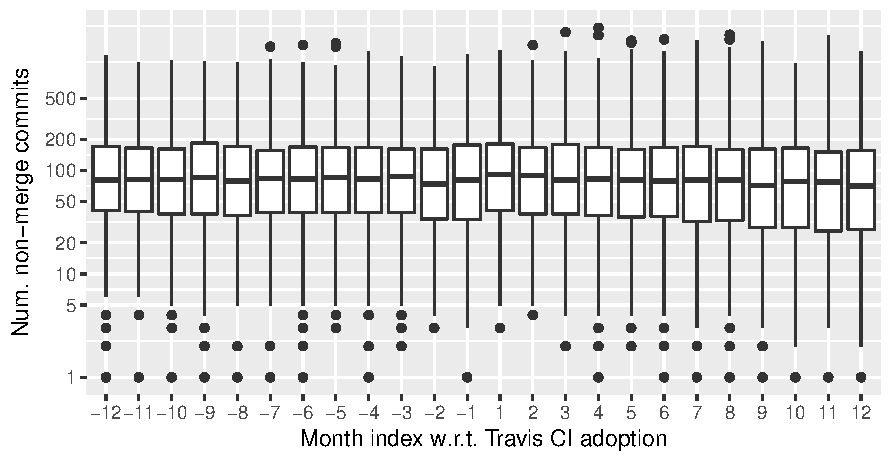
\includegraphics[width=\columnwidth, clip=true, trim=0 0 0 32]{figures/freq-non-merge.pdf}
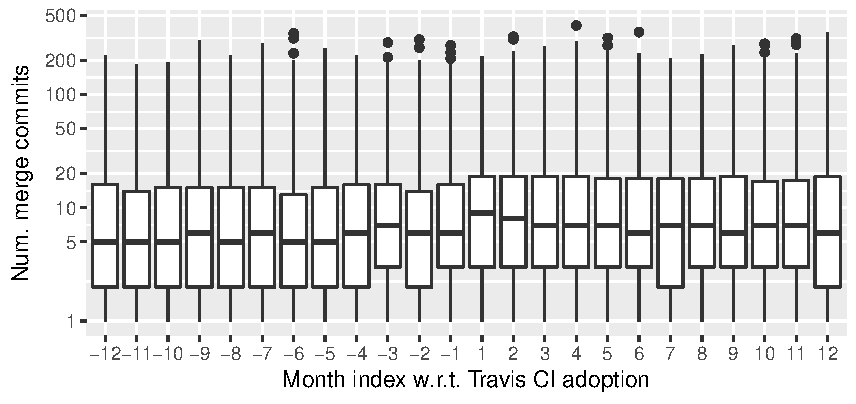
\includegraphics[width=\columnwidth, clip=true, trim=0 0 0 0]{figures/freq-merge.pdf}
\caption{Commit frequency before and after the \Tvis adoption.}
\label{fig:freq}
\end{figure}


\subsection{RQ1: Trends in Commit Frequency}

%Starting from RQ1 and RQ2 the practice being investigate should be �Commits To the Mainline Every Day�, but then you analyze git commits. Not surprisingly, commits do not increase. Why they should? The main reason of having many commits is the ability to partition a large change in many smaller ones and to better handle the work locally. What really matters for the CI are pushes and pull/requests. Indeed, I would expect an increase of pushes/pull requests when CI is being adopted. Maybe a way to observe this is to actually analyze merge commits and see whether their frequency increases.
%Similar considerations apply for the size of code changes. Also, I�ve the feeling that such a size may strongly depend on the kind of activity being performed. For example, it could be that bug fixing correlates with small change size, whereas feature addition with larger ones. Unfortunately, such a factor is not controlled.


The first practice we examine is commit frequency.
As we investigate the ``Commits to the Mainline Every Day'' practice, it is
important to distinguish non-merge from merge commits.
Indeed, local git commits, in a developer's offline repository, happen in 
isolation and can be seen as simply a mechanism to partition the work.
However, what matters for \Tvis are pushes and pull requests to the blessed 
\GH repository, \ie only then \Tvi would be triggered.
Push events are not readily accessible in our data, hence we analyze 
merge commits on the main development branch as a proxy for work
that would have been subjected to CI by \Tvi.
Since not all our projects have recorded merge commits in \emph{all} 24 
periods, we restrict this analysis to only 575 projects that had at least one 
merge commit in each time window.

%(we obtained the latter as described previously in the Methods section).


%We started from the same data as before, 567 projects, each with at least 500 
%non-merge commits.
%Additionally, we restricted the projects for the  merge commits study so that we only look at projects that have at least 20 merge commits over the 18 time points, \ie on average about 1 per time point.
%This filtering yielded a set of 370 projects for the merge commit frequency study.

%\begin{figure}[!t]
%\centering
%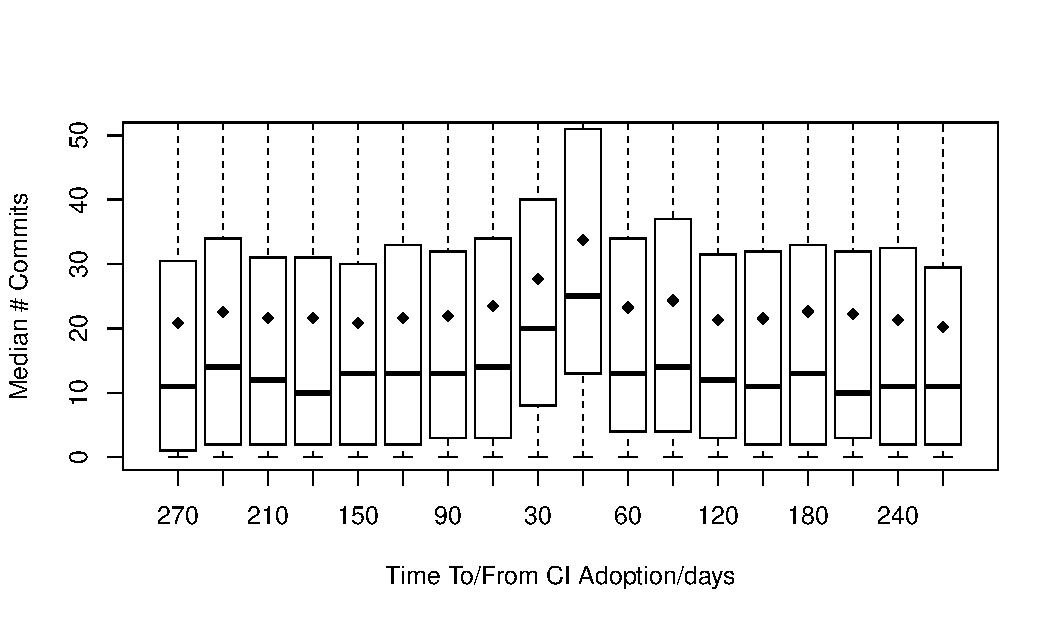
\includegraphics[width=0.45\textwidth, clip=true, trim=0 15 15 50]{numbercommits.pdf}
%\caption{Non-merge commit frequency before and after CI adoption}
%\label{Fig:NumberCommits}
%\end{figure}
%
%\begin{figure}[!t]
%\centering
%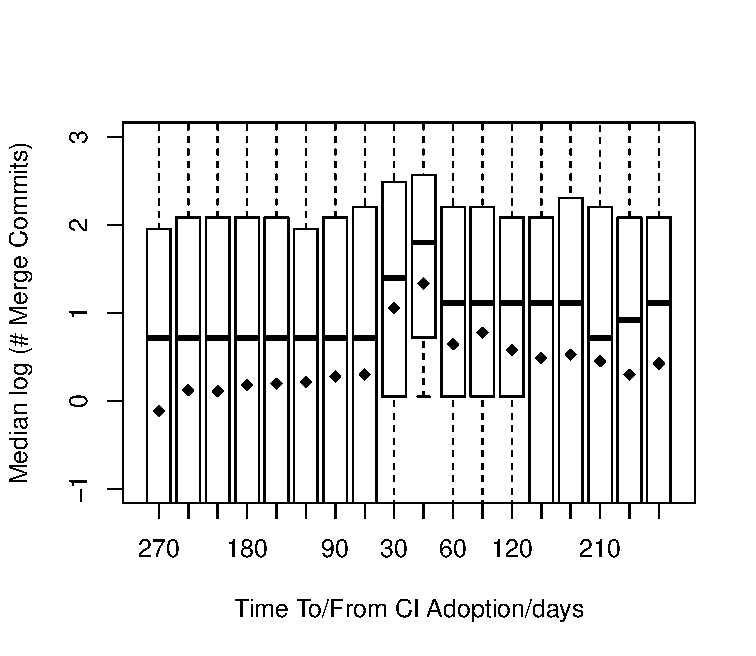
\includegraphics[width=0.45\textwidth, height=1.5in, clip=true, trim=0 15 15 50]{merges.pdf}
%\caption{Merge commit frequency before and after CI adoption}
%\label{Fig:MergeCommits}
%\end{figure}

\smallskip\noindent \emph{Exploratory Study}: 
Figure~\ref{fig:freq} shows the boxplots of per-project number of non-merge 
commits (top) and number of merge commits (bottom), respectively, for each
of twelve consecutive 30-day time intervals before and after the \Tvis adoption.
Note the log scale.
Recall that due to instability, we omit the 30-day time interval centered 
around $t = 0$, when the earliest commit to the \Tvi configuration file, which 
signals adoption, was recorded (Figure~\ref{fig:timeseries}).
The horizontal line in each boxplot is the median value across all projects.

First, we observe relative stability in the number of non-merge commits prior 
to the \Tvis adoption (Figure~\ref{fig:freq}, top), with the across-projects medians 
around 78 commits, and a slight decreasing trend after the adoption, with the
across-projects median dropping to 67 commits in period 12.
Second, after an initial dip in periods -12 to -10, the merge commits 
(Figure~\ref{fig:freq}, bottom) appear to display a slight increasing trend prior 
to the \Tvis adoption, with the across-projects median reaching 18 commits 
immediately prior to the adoption period, followed by apparent stabilization 
after that.
We also observe a discontinuity at $t=0$: the across-projects median is 21 
commits right after the adoption period.
Note, in both plots, the large variance in the data.

%To explore general trends over time, we first look at commit frequency in 
%the months leading up to CI adoption.
%Figs.~\ref{Fig:NumberCommits} and \ref{Fig:MergeCommits} show the boxplots 
%of per-project median number of non-merge commits, and merge commits, 
%respectively, for each of nine consecutive 30-day time intervals before CI adoption 
%and, respectively, nine consecutive 30-day time intervals after CI adoption.
%We use a log-scale for the merge commits due to the overdispersion of the data 
%which is sparse over the time periods we have chosen.
%As before, the horizontal line in each boxplot is the median value of all 
%per-project medians, and the black dot is their average value.

%As with code churn, here we also see a peak in the 30-day 
%interval just before and the one just after CI adoption.
%We do not observe an apparent trend in the 
%median or average non-merge commit frequency.
%We do observe an upward trend in merge commits, but the variance in the data is large.

\smallskip\noindent \emph{Statistical Modeling Study}: 
We fitted a mixed-effects RDD model, as described before, to model trends
in the \emph{number of merge commits} per project, over time, as a function 
of \Tvis adoption, and while controlling for confounds; most notably, we control 
for the \emph{number of non-merge commits}, as these may have not all been 
subjected to CI, since they appear to display a decreasing trend with time.


 

\begin{table}[t]
\centering 
\footnotesize
\rowcolors{3}{Gray}{}
\begin{tabular}{l D{)}{)}{13)3}@{} D{.}{.}{5.5} }
\hline
                                               & \multicolumn{1}{c}{Coeffs (Errors)} & \multicolumn{1}{c}{Sum Sq.} \\
\hline
(Intercept)                            & -0.958 \; (0.232)^{***} & \\
log(TotalCommits)                      & -0.016 \; (0.032)     & 0.07  \\
log(NumNonMergeCommits)          & 0.777 \; (0.007)^{***} & 3095.91^{***} \\
AgeAtTravis                            & -0.001 \; (0.001)      & 0.96 \\
log(NumAuthors)                        & 0.120 \; (0.026)^{***} & 5.67^{***} \\
time                                   & 0.019 \; (0.002)^{***} & 30.39^{***} \\
interventionTRUE                       & -0.024 \; (0.027)      & 0.21 \\
time\_after\_intervention              & -0.016 \; (0.003)^{***} & 10.96^{***}\\
\hline
%AIC                                    & 24086.065               \\
%BIC                                    & 24183.986               \\
%Log Likelihood                         & -12030.032              \\
%Num. obs.                              & 13800                   \\
%Num. groups: Repo                      & 575                     \\
%Num. groups: Language                  & 21                      \\
%Var: Repo (Intercept)                  & 0.413                   \\
%Var: Repo interventionTRUE             & 0.207                   \\
%Cov: Repo (Intercept) interventionTRUE & -0.121                  \\
%Var: Language (Intercept)              & 0.001                   \\
%Var: Residual                          & 0.270                   \\
\hline
\rowcolor{white}
\multicolumn{2}{l}{\scriptsize{$^{***}p<0.001$, $^{**}p<0.01$, $^*p<0.05$}}
\end{tabular}
\caption{Commit frequency model. The response is \textbf{log(number of merge commits)}
per month. $R^2_m = 0.58$. $R^2_c = 0.83$.}\vspace{-0.5cm}
\label{table:freq}
\end{table}

%> r.squaredGLMM(m1)
%      R2m       R2c 
%0.5828560 0.8311715 
%> vif.mer(m1)
%         log(TotalCommits) log(num_non_merge_commits)                AgeAtTravis            log(NumAuthors)                       time           interventionTRUE 
%                  1.774990                   1.082181                   1.311646                   1.396992                   3.266075                   1.634289 
%   time_after_intervention 
%                  2.641925 
%> anova(m1)
%Analysis of Variance Table of type III  with  Satterthwaite 
%approximation for degrees of freedom
%                            Sum Sq Mean Sq NumDF   DenDF F.value    Pr(>F)    
%log(TotalCommits)             0.07    0.07     1   631.5     0.2   0.61990    
%log(num_non_merge_commits) 3095.91 3095.91     1 13519.1 11474.7 < 2.2e-16 ***
%AgeAtTravis                   0.96    0.96     1   394.1     3.6   0.05984 .  
%log(NumAuthors)               5.67    5.67     1   563.3    21.0 5.576e-06 ***
%time                         30.39   30.39     1 12647.3   112.6 < 2.2e-16 ***
%intervention                  0.21    0.21     1  1506.5     0.8   0.37626    
%time_after_intervention      10.96   10.96     1 12652.0    40.6 1.909e-10 ***
%
 

\begin{table}[t]
\caption{Commit frequency model. The response is \textbf{log(number of non-merge commits)}
per month. $R^2_m = 0.57$. $R^2_c = 0.77$.}
\label{table:freq} 
\centering \footnotesize
\rowcolors{3}{Gray}{}
\begin{tabular}{l D{)}{)}{13)3}@{} D{.}{.}{5.5} }
\hline
                                               & \multicolumn{1}{c}{Coeffs (Errors)} & \multicolumn{1}{c}{Sum Sq.} \\
\hline
(Intercept)                            & -1.660 \; (0.102)^{***} & \\
log(TotalCommits)                      & 0.662 \; (0.015)^{***} & 933.1^{***}  \\
log(num\_merge\_commits+1)           & 0.558 \; (0.004)^{***} & 8323.6^{***} \\
AgeAtTravis                            & -0.003 \; (0.000)^{***} & 30.7^{***}\\
log(NumAuthors)                        & -0.215 \; (0.011)^{***} & 173.2^{***}\\
time                                   & -0.012 \; (0.001)^{***} & 40.8^{***}\\
interventionTRUE                       & 0.102 \; (0.018)^{***} & 15.1^{***} \\
time\_after\_intervention              & -0.013 \; (0.002)^{***} & 25.5^{***}\\
\hline
%AIC                                    & 111917.158              \\
%BIC                                    & 112031.638              \\
%Log Likelihood                         & -55945.579              \\
%Num. obs.                              & 49323                   \\
%Num. groups: Repo                      & 2401                    \\
%Num. groups: Language                  & 22                      \\
%Var: Repo (Intercept)                  & 0.399                   \\
%Var: Repo interventionTRUE             & 0.339                   \\
%Cov: Repo (Intercept) interventionTRUE & -0.178                  \\
%Var: Language (Intercept)              & 0.010                   \\
%Var: Residual                          & 0.462                   \\
\hline
\rowcolor{white}
\multicolumn{2}{l}{\scriptsize{$^{***}p<0.001$, $^{**}p<0.01$, $^*p<0.05$}}
\end{tabular}
\end{table}



Recall that we modeled a random intercept for \emph{programming language}, 
to allow for language-to-language variability in the response (\ie code in some 
languages being naturally more verbose than in others, resulting in different
ways to split the work across commits; or community-level norms for committing), 
and a random \emph{intervention} slope and intercept for \emph{project}, to allow 
for project-to-project variability in the response and the possibility that, on average, 
projects with lower initial activity may be less strongly affected by adopting 
\Tvis than high-frequency projects.
Recall also that the coefficient for \emph{time} is the slope before adoption,
the coefficient for \emph{intervention} is the size of the effect of CI introduction,
the coefficient for \emph{time after intervention} is the divergence in the slopes
before and after \Tvis adoption, and the sum of the coefficients for \emph{time}
and \emph{time after intervention} is the slope of the linear trend after \Tvis
adoption.

Table~\ref{table:freq} summarizes the results.
In addition to the model coefficients and corresponding standard errors, the table 
shows the sum of squares, a measure of variance explained, for each variable.
The statistical significance is indicated by stars.
The fixed-effects part of the model fits the data well ($R_m^2=0.58$).
There is also a considerable amount of variability explained by the random
effects, \ie project-to-project and language-to-language differences, not 
explicitly modeled by our fixed effects ($R_c^2=0.83$).
Among the fixed effects, we observe that the \emph{number of non-merge 
commits}, our main control, explains most of the variability in the response.
The coefficient is positive, \ie the direction of the correlation is expected: 
other things constant, the more non-merge commits there are, the more 
merge commits there will be as well.
Neither \emph{project size} (total number of commits over the entire history) nor 
\emph{project age} at adoption time have any statistically significant effects.

Next we turn to our \Tvi-related variables.
The model confirms a statistically significant, positive, baseline trend in the response 
with \emph{time} (with a small effect), as suggested by our exploratory study.
The model does not detect any discontinuity at adoption time, since the coefficient 
for \emph{intervention} is not statistically significant.
Post adoption, there is a decrease in the slope of the time trend, but the overall 
trend remains ascending (the sum of the coefficients for \emph{time} and 
\emph{time after intervention} is positive): more merge-commits as time passes.

%As before, we eliminated one time point on either side of the CI adoption 
%time, so that the peaks at those times  do not throw off the regression models.
%% !TEX root = ../CI_Adoption.tex

\begin{table}[t] \centering
\small
  \caption{Model Coefficients for 567 Models of Commit Frequency}
  \label{Table:rddmodels_freq}
\begin{tabular}{ l  r r r r }        
\hline 

 & $\beta$ & $\gamma$ & $\delta$ & $\beta + \delta$ \\ 
 \hline 
 \hline
not signif. & 452 & 466 & 454 & \\
\hline
signif., $\ge 0$ & 71 & 59 & 33 & 42 \\
\hline
signif., $<0$ & 44 & 42 & 80 & 71 \\
\hline
\end{tabular}
\end{table}

\begin{table}[t] \centering
\small
  \caption{Model Coefficients for 370 Models of Merge Commit Frequency}
  \label{Table:rddmodels_merge_freq}
\begin{tabular}{ l  r r r r }        
\hline 

 & $\beta$ & $\gamma$ & $\delta$ & $\beta + \delta$ \\ 
 \hline 
 \hline
not signif. & 296 & 307 & 301 & \\
\hline
signif., $\ge 0$ & 46 & 35 & 26 & 44 \\
\hline
signif., $<0$ & 28 & 28 & 43 & 30 \\
\hline
\end{tabular}
\end{table}

%For the non-merge commits, in 452 (80\%) of the models, there was no significant linear relationship 
%between  frequency and time, \ie there was no linear trend.
%In 71 projects there was a rising trend in commit frequency before CI 
%and in 44 projects a falling trend before CI.
%Similarly, in 466 projects no effect of CI introduction on commit frequency 
%was found. 
%Among the 101 projects where an effect was significant, in 59 the trend 
%was positive, \ie commit frequency increased, and in the rest it was 
%negative, \ie commit frequency decreased.
%The mean value over all projects for $\gamma$, the effect size of CI 
%adoption, was $1.1$ commit.
%While in 454 projects no change of slope in the trends before and after CI 
%adoption was found, in the 113 with significant change of trends a reduction 
%in the slope was more prevalent than an increase by about 2.5 to 1.
%This carried over to a lesser degree into trends in commit frequency 
%following CI adoption: out of the 113 significant trend changes, 71 are 
%downward trends, and 42 are upward.
%
%For merge commits (Table~\ref{Table:rddmodels_merge_freq}), the results 
%are qualitatively similar to those for non-merge commits.

\smallskip\noindent \emph{Discussion}:
The exploratory study suggests a slight decreasing trend in the number 
of non-merge commits with time.
Separately modeling the trend in \emph{number of non-merge commits}
(not shown) using a similar approach as above confirmed this overall 
decreasing trend.
This is consistent with the common observation that, as projects move 
past the initial development hurdle and age, development generally slows 
down, and the focus shifts to bug-fixing rather than adding new features, 
noted, \eg by Brindescu \etal~\cite{brindescu2014centralized}.

In contrast, the statistical modeling study above revealed a consistent 
increase in \emph{merge commits} with time, including post-CI adoption, 
albeit with a slowdown.
This overall trend aligns with the expected increase in commit frequency 
after switching to CI, as expressed and encouraged by Fowler.
Given the overall decreasing trend with time in the number of non-merge
commits, the increase in merge commits is noteworthy.
One explanation is that projects are switching to more distributed
development workflows, using branches and pull requests. 
Indeed, in our survey, R38 has indicated that their project ``shifted towards 
pull-request - merge development strategy as it made the distributed 
development more manageable.''
The development process change reported by R38 is not exceptional. 
Indeed, the idea of a shift towards more focused development in separated 
branches has been voiced by R32 (``shorter lived (and generally single contributor) 
branches'') and R49 (``feature branches''), R6, and R47.
% both report more 
%emphasis on branches.
%R6 speaks of ``much more emphasis'' being put on using 

%\as{R38 The release process got changed. Additionally we have shifted towards pull-request - merge development strategy. It made the distributed development more manageable.}
%\as{R44 develop branch is more stable; we can trust it more and release sooner}
%\as{R46 Regular releases \& work on development branch}
%\as{R54 We've moved as much as possible into CI (eg doc generation, building release artifacts, etc.).}

%As was the case for code churn, most projects did not have longitudinal 
%linear trends in non-merge commits, for reasons probably similar to those 
%in case of code churn.

%We observed a post-CI adoption increase in merge commits 

%in our exploratory study, the statistical tests did not confirm that to be the 
%case for more than 20\% of the projects. 
%We attribute this disparity to the large variance in the data and especially 
%the sparsity of merge commits over time. 
%
%While our exploratory study did not suggest presence of a trend, the 
%modeling study suggests that right after CI adoption there is a slight 
%positive effect in both the merge and non-merge commits (after removing the peak months around CI adoption time). 
%However, this effect is not sustained.
%% if a linear trend is present, which is 2.5 times as likely to be decreasing as increasing. 

%Given the expected increase in the frequency of commits expressed and 
%encouraged by Fowler, our results might appear surprising.
%It is possible that some saturation to the commit frequency has already 
%been reached even before the CI adoption time.
%As we see next, it is also likely that instead developers are spending more time on 
%automated testing.




\subsection{RQ2: Trends in Code Churn}

The next development practice we examine is code churn.
%Recall that our data consists of \bv{2,401 projects across 22 programming languages.}
We distinguish between merge and non-merge commits.

\begin{figure}[t]
\centering
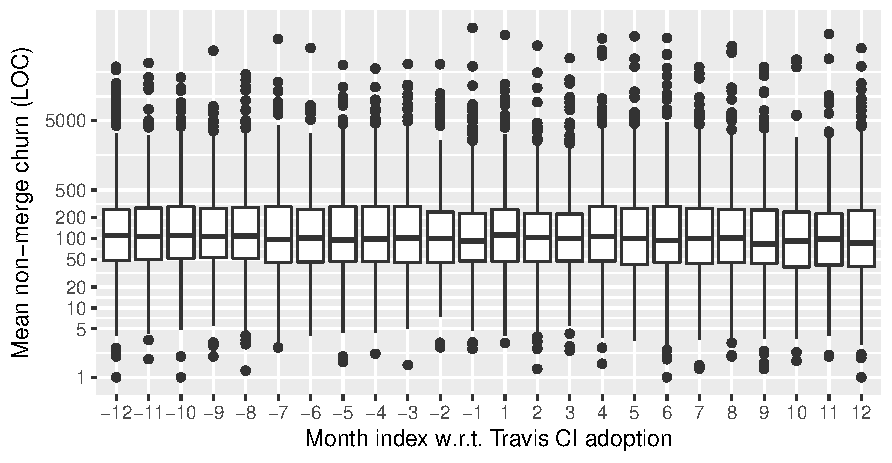
\includegraphics[width=\columnwidth, clip=true, trim=0 0 0 0]{figures/churn-non-merge.pdf}
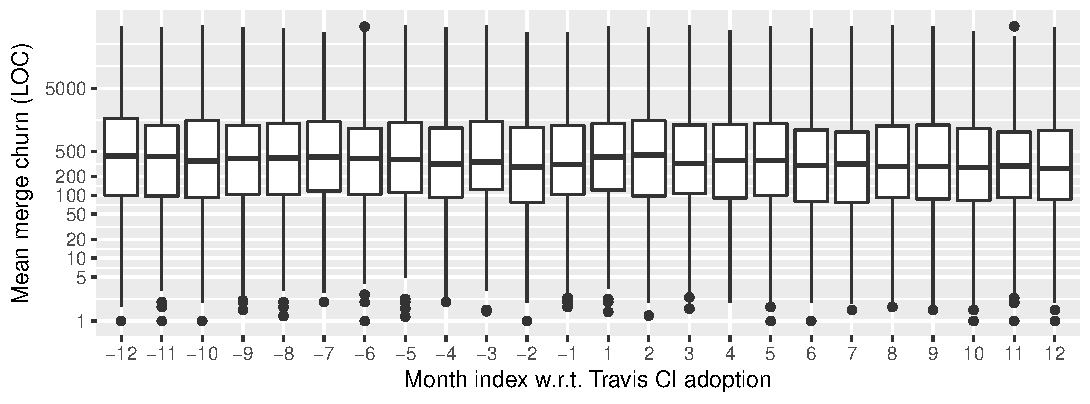
\includegraphics[width=\columnwidth, clip=true, trim=0 0 0 0]{figures/churn-merge.pdf}
\caption{Mean code churn per commit per project, before and after \Tvi.}
\label{fig:churn}
\end{figure}

\smallskip\noindent \emph{Exploratory Study}: 
Figure~\ref{fig:churn} shows boxplots of per-project per-commit mean code 
churn (medians behave similarly) for each of twelve consecutive 30-day time 
intervals before, and after, the \Tvis adoption.
The horizontal line in each boxplot is the median value over all projects.

We observe that, in the non-merge commits, the medians are quite stable
across the entire interval, from before to after the \Tvis adoption, dancing 
around 100 
% pre-\Tvi, the medians are quite stable, dancing around 65 
lines of code churn per commit on average, with large variance.
%The 30-day interval just before \Tvis adoption (-1) seems to stand out and is 
%slightly higher than the rest (median = 73 LOC), as is the 30-day interval just after 
%\Tvi (1).
In comparison, in the merge-commits, we observe more than usual variance
in the two months preceding the adoption, as well as a slight downward trend 
%On the other side, following \Tvis adoption, 
in the medians following adoption, which drop to about 263 lines of code churn 
per commit on average in the last period (12), compared to about 405 right after 
adoption (period 1).
However, we again note the large variance around the medians in all periods.

In conclusion, non-merge commits seem mostly unaffected by time passing and 
the \Tvis adoption, while merge commits seem to be getting smaller with time.
%discounting the peak behavior in code churn around adoption time, 
%we observe a small reduction in the amounts of code churn from before 
%to after the adoption.

%To explore general trends over 
%time, we first look at code churn in months leading up to CI adoption.
%The horizontal line in each boxplot is the median value of all per-project medians, 
%and the black dot is their average value.
%We observe that, for most part, the medians dance around 10 and 12 lines of 
%code churn per period, and the averages between 16 and 18 lines, with large 
%variance and no obvious trend. 
%The 30-day interval just before CI adoption seems to stand out and is higher 
%than the rest.

%Next, we look to the other side of the adoption point. 
%Fig.~\ref{Fig:CodeChurnAfter} shows a boxplot of per-project median code 
%churn for each of nine consecutive 30-day time intervals following CI adoption.
%Here, there seems to be a slight downward trend in both the medians and 
%averages; the former drop monotonically from 13 down to 8 lines of code and 
%the latter down to 15 lines of code.
%However, we note the large variance around the medians.

%The 30- and 60-day intervals just after the adoption point seem to be higher 
%than the rest, and together with the 30-day interval just before adoption of CI 
%seem to form a peak of increased code churn.
%In conclusion, discounting the peak behavior in code churn around CI adoption 
%time, we observe a small reduction in the amounts of code churn from before 
%to after CI adoption.

%% !TEX root = ../CI_Adoption.tex

\begin{table}[t] \centering
\small
  \caption{Model Coefficients for 566 Models of Code Churn}
  \label{Table:rddmodels}
\begin{tabular}{ l  r r r r }        
\hline 

 & $\beta$ & $\gamma$ & $\delta$ & $\beta + \delta$ \\ 
 \hline 
 \hline
not signif. & 504 & 508 & 514 & \\
\hline
signif., $>0$ & 45 & 28 & 10 & 13 \\
\hline
signif., $<0$ & 17 & 30 & 42 & 39 \\
\hline
\end{tabular}
\end{table}

 

\begin{table}[t]
\centering \footnotesize
\rowcolors{3}{Gray}{}
\begin{tabular}{l D{)}{)}{13)3}@{} D{.}{.}{5.5} }
\hline
                                               & \multicolumn{1}{c}{Coeffs (Errors)} & \multicolumn{1}{c}{Sum Sq.} \\
\hline
(Intercept)                            & 1.311 \; (0.132)^{***} & \\
log(TotalCommits)                      & 0.439 \; (0.016)^{***}  & 588.51^{***} \\
AgeAtTravis                            & -0.003 \; (0.000)^{***} & 48.10^{***} \\
log(NumAuthors)                        & -0.173 \; (0.012)^{***} & 158.77^{***} \\
time                                   & 0.002 \; (0.002)       & 0.93 \\ 
interventionTRUE                       & 0.039 \; (0.019)^{*}    & 3.22^{*} \\
time\_after\_intervention              & -0.023 \; (0.002)^{***} & 75.59^{***} \\
%
%
%(Intercept)                                & 1.125 \; (0.161)^{***}  &  \\
%log(TotalCommits)                          & 0.514 \; (0.020)^{***}  & 588.51^{***} \\
%AgeAtTravis                                & -0.003 \; (0.001)^{***} & 48.10^{***} \\
%log(NumAuthors)                            & -0.218 \; (0.016)^{***} & 158.77^{***} \\
%time                                       & 0.002 \; (0.002)       & 0.93 \\
%interventionTRUE                           & 0.072 \; (0.028)^{**}  & 3.22^{*} \\
%time\_after\_intervention                  & -0.024 \; (0.003)^{***} & 75.59^{***} \\
%(Intercept)                                          & 0.069 \; (0.012)^{***}   & \\
%GlobalTime                                    & -0.037 \; (0.005)^{***}  & 15.71^{***} \\
%Projects                                      & 0.263 \; (0.006)^{***}   & 2566.87^{***} \\
%Languages                                     & 0.549 \; (0.004)^{***}   & 11505.20^{***} \\
%$S_\text{Focus}$                                  & -0.300 \; (0.004)^{***}  & 2757.75^{***} \\
%$S_\text{Language}$                               & -0.231 \; (0.003)^{***}  & 2354.39^{***} \\
%AvgProjectsPerDay                             & 0.046 \; (0.004)^{***}   & 215.29^{***} \\
%$S_\text{Switch}$                          & 0.225 \; (0.004)^{***}   & 2255.09^{***} \\
%Projects:$S_\text{Focus}$                  & 0.032 \; (0.003)^{***}   & 0.16^{***} \\
%Languages:$S_\text{Language}$              & -0.045 \; (0.002)^{***}  & 345.96^{***} \\
%Projects:$S_\text{Language}$               & -0.021 \; (0.003)^{***}  & 68.66^{***} \\
%Projects:AvgProjectsPerDay             & -0.024 \; (0.003)^{***}  & 128.60^{***} \\
%$S_\text{Language}$:AvgProjectsPerDay      & 0.026 \; (0.003)^{***}   & 59.86^{***} \\
%Projects:$S_\text{Switch}$          & -0.104 \; (0.003)^{***}  & 404.80^{***} \\
%AvgProjectsPerDay:$S_\text{Switch}$ & 0.058 \; (0.003)^{***}   & 203.12^{***} \\
%$S_\text{Language}$:$S_\text{Switch}$   & -0.029 \; (0.003)^{***}  & 35.99^{***} \\
\hline
%\multicolumn{3}{c}{AIC = 175178.307; BIC =  175303.204; LogLik = -87575.153           }                                          \\
%\rowcolor{white}
%\rowcolor{white}
%\multicolumn{3}{c}{Num. obs. = 55340; Num. groups: Repo = 2405; Language = 22}\\
%AIC                                        & 175178.307              \\
%BIC                                        & 175303.204              \\
%Log Likelihood                             & -87575.153              \\
%Num. obs.                                  & 55340                   \\
%Num. groups: Repo                          & 2405                    \\
%Num. groups: Language                      & 22                      \\
%Var: Repo (Intercept)                      & 0.666                   \\
%Var: Repo interventionTRUE                 & 0.262                   \\
%Cov: Repo (Intercept) interventionTRUE     & -0.138                  \\
%Var: Language (Intercept)                  & 0.145                   \\
%Var: Language interventionTRUE             & 0.003                   \\
%Cov: Language (Intercept) interventionTRUE & 0.002                   \\
%Var: Residual                              & 1.200                   \\
%Analysis of Variance Table of type III  with  Satterthwaite 
%approximation for degrees of freedom
%                        Sum Sq Mean Sq NumDF DenDF F.value    Pr(>F)    
%log(TotalCommits)       760.54  760.54     1  2412  634.04 < 2.2e-16 ***
%AgeAtTravis              49.73   49.73     1  2386   41.46 1.449e-10 ***
%log(NumAuthors)         234.13  234.13     1  2373  195.19 < 2.2e-16 ***
%time                      0.77    0.77     1 50696    0.65   0.42188    
%intervention              8.29    8.29     1    11    6.91   0.02413 *  
%time_after_intervention  95.91   95.91     1 50681   79.96 < 2.2e-16 ***
%---
%Signif. codes:  0 �***� 0.001 �**� 0.01 �*� 0.05 �.� 0.1 � � 1
\hline
\rowcolor{white}
\multicolumn{2}{l}{\scriptsize{$^{***}p<0.001$, $^{**}p<0.01$, $^*p<0.05$}}
\end{tabular}
\caption{Commit churn model. The response is \textbf{log(mean commit churn)}
per month. $R^2_m = 0.1$. $R^2_c = 0.46$.}
\label{table:churn}
 
\end{table}



 

\begin{table}[t]
\caption{Commit churn model 2. The response is \textbf{log(mean merge-commit churn)}. $R^2_m = 0.20$. $R^2_c = 0.51$.}
\label{table:churn:merge}
\centering \footnotesize
\rowcolors{3}{Gray}{}
\begin{tabular}{l D{)}{)}{13)3}@{} D{.}{.}{5.5} }
\hline
                                               & \multicolumn{1}{c}{Coeffs (Errors)} & \multicolumn{1}{c}{Sum Sq.} \\
\hline
(Intercept)                            & -1.297 \; (0.484)^{**}  \\
log(TotalCommits)                      & 1.113 \; (0.062)^{***} & 625.20^{***}  \\
AgeAtTravis                            & -0.005 \; (0.001)^{**} & 18.43^{**} \\
log(NumAuthors)                        & -0.522 \; (0.052)^{***} & 196.48^{***} \\
time                                   & -0.012 \; (0.005)^{*}  & 8.86^{*} \\
interventionTRUE                       & 0.220 \; (0.066)^{***} & 21.75^{***} \\
time\_after\_intervention              & -0.022 \; (0.008)^{**} & 15.51^{**} \\
\hline


%Analysis of Variance Table of type III  with  Satterthwaite 
%approximation for degrees of freedom
%                        Sum Sq Mean Sq NumDF   DenDF F.value    Pr(>F)    
%log(TotalCommits)       625.20  625.20     1   459.7  319.85 < 2.2e-16 ***
%AgeAtTravis              18.43   18.43     1   464.7    9.43 0.0022600 ** 
%log(NumAuthors)         196.48  196.48     1   460.7  100.52 < 2.2e-16 ***
%time                      8.86    8.86     1 10136.0    4.53 0.0332503 *  
%intervention             21.75   21.75     1  2384.4   11.13 0.0008638 ***
%time_after_intervention  15.51   15.51     1 10134.2    7.94 0.0048571 ** 

%AIC                                    & 40504.501               \\
%BIC                                    & 40592.239               \\
%Log Likelihood                         & -20240.250              \\
%Num. obs.                              & 11065                   \\
%Num. groups: Repo                      & 467                     \\
%Num. groups: Language                  & 7                       \\
%Var: Repo (Intercept)                  & 1.145                   \\
%Var: Repo interventionTRUE             & 0.530                   \\
%Cov: Repo (Intercept) interventionTRUE & -0.272                  \\
%Var: Language (Intercept)              & 0.087                   \\
%Var: Residual                          & 1.955                   \\


%(Intercept)                            & -1.308 \; (0.426)^{**} & \\
%log(TotalCommits)                      & 1.131 \; (0.057)^{***} & 795.76^{***}  \\
%AgeAtTravis                            & -0.004 \; (0.001)^{**}  & 14.06^{**}\\
%log(NumAuthors)                        & -0.583 \; (0.048)^{***} & 302.31^{***}\\
%time                                   & -0.011 \; (0.005)^{*}   & 10.07^{*}\\
%interventionTRUE                       & 0.207 \; (0.061)^{***}  & 23.93^{***}\\
%time\_after\_intervention              & -0.018 \; (0.007)^{*}   & 13.11^{*}\\
%\hline
%AIC                                    & 51186.198               \\
%BIC                                    & 51276.582               \\
%Log Likelihood                         & -25581.099              \\
%Num. obs.                              & 13794                   \\
%Num. groups: Repo                      & 575                     \\
%Num. groups: Language                  & 21                      \\
%Var: Repo (Intercept)                  & 1.218                   \\
%Var: Repo interventionTRUE             & 0.560                   \\
%Cov: Repo (Intercept) interventionTRUE & -0.290                  \\
%Var: Language (Intercept)              & 0.103                   \\
%Var: Residual                          & 2.056                   \\
\hline
\rowcolor{white}
\multicolumn{2}{l}{\scriptsize{$^{***}p<0.001$, $^{**}p<0.01$, $^*p<0.05$}}
\end{tabular}
\end{table}



\smallskip\noindent \emph{Statistical Modeling Study}: 
Guided by our exploratory observations above, we proceed to quantify the 
trends we observed using two mixed-effects RDD models, for non-merge 
and merge commits, respectively, as described before.
%Recall that we modeled a random intercept for \emph{programming language}, 
%to allow for language-to-language variability in the response (\ie code in some 
%languages being naturally more verbose than in others), and a random 
%\emph{intervention} slope and intercept for \emph{project}, to allow for 
%project-to-project variability in the response, and the possibility that, on average, 
%projects with lower initial churn values may be less strongly affected by adopting 
%\Tvis, since their commits are already ``small enough'' for efficient CI.
%Recall also that the coefficient for \emph{time} is the slope before adoption,
%the coefficient for \emph{intervention} is the size of the effect of CI introduction,
%the coefficient for \emph{time\_after\_intervention} is the divergence in the slopes
%before and after \Tvis adoption, and the sum of the coefficients for \emph{time}
%and \emph{time\_after\_intervention} is the slope of the linear trend after \Tvis
%adoption.

Table~\ref{table:churn} summarizes the RDD model for non-merge commits.
%In addition to the model coefficients and corresponding standard errors, the table 
%shows the sum of squares, a measure of variance explained, for each variable.
%The statistical significance is indicated by stars.
First, we observe that only the combined fixed-and-random effects model fits the 
data well ($R_c^2 = 0.48$ compared to $R_m^2 = 0.09$), \ie most of the explained 
variability in the data is attributed to project-to-project and language-to-language
variability, rather than any of the fixed effects, either controls or RDD-related.

Next, we turn to the fixed effects.
From among the controls, we note that overall bigger projects (\emph{TotalCommits}) 
tend to churn more, other things held constant; and projects with a larger contributor 
base (\emph{NumAuthors}), which typically indicate many occasional contributors, 
also tend to churn less.
None of the \Tvi-related predictors have statistically significant effects,
%, except for
%\emph{time\_after\_intervention}, which has a negative coefficient with a small 
%effect; 
\ie the churn trend in non-merge commits is stationary over time, and 
remains unaffected by the \Tvis adoption.

Table~\ref{table:churn:merge} summarizes the RDD model for merge commits.
Similarly as with the previous model of churn in non-merge commits, most of 
the explained variability in the data is attributed to project-to-project and 
language-to-language variability, rather than any of the fixed effects variables.
The controls also behave similarly as before: older projects tend to churn less, 
perhaps as they have reached maturity and a more stationary stage in their 
evolution; projects with a larger contributor base also tend to churn less, which 
is in line with the expectation that occasional contributors to open source projects 
are generally less active than core developers; small pull request contributions
would be reflected here.

After controlling for confounds, we move on to the main time series predictors,
all of which now have statistically significant effects.
The coefficient for \emph{time} is negative, suggesting a small decreasing
baseline trend in commit churn before CI adoption; the \emph{intervention}
coefficient signals a discontinuity in the time series at the time of the \Tvis
adoption; the negative coefficient \emph{time\_after\_intervention} signals
an acceleration in the baseline trend.
Taken together, this confirms a change in merge commit churn at the time 
of adoption, followed by an accelerated decreasing trend after adopting \Tvis.

%not statistically significant, 
%\ie there is no baseline trend in commit churn before CI adoption, and the 
%\emph{intervention}, although statistically significant, has a small effect.
%However, \emph{time\_after\_intervention} has a statistically significant, 
%negative coefficient, with a notable effect size.


\smallskip\noindent \emph{Discussion}:
%Across our sample, %\bv{(2,401 projects across 22 programming languages)},
Our modeling study revealed a statistically significant discontinuity
in the merge commit churn time series when adopting \Tvis; and a statistically 
significant decreasing linear trend with time in merge commit churn after adopting \Tvis.
However, churn in non-merge commits remains unaffected by either time or 
switching to \Tvis.

The discontinuity is not unexpected, as one can reasonably expect more 
maintenance work in preparation for transitioning to \Tvis, 
and some adjustment/cleanup period right after.
The relative instability in code churn on both sides near the CI adoption time is 
also indication of this, as are the survey results.  
Indeed, when asked about the introduction of \Tvis, respondents frequently refer 
to test automation being introduced around the same time as \Tvi ``as contributors 
couldn't be trusted to run test suite on their own'' (R25). Furthermore, respondents 
indicate that \Tvi has been introduced as ``a part of automated package/release 
effort'' (R38) and to ``deploy artifacts to S3 on each commit, as part of our 
deployment process using Amazon CodeDeploy'' (R34).

The decreasing trend in code churn post \Tvi is visible only among merge commits,
which are more likely to be affected by switching to a fast-paced CI workflow than
non-merge commits, which may live on local, isolated developer branches for
some time before being merged to the remote.
This finding is consistent with Fowler's recommended good practices of CI, of 
committing smaller changes to the code.
The expected decrease in the size of the commits is also echoed by one of the 
survey respondents: ``commits became smaller and more frequent, to check 
the build; pull requests became easier to check'' (R4).
However, the decreasing trend we observed is not particularly steep.
Survey responses provide a possible explanation: several developers 
referred to pull request integration as the reason for introducing \Tvis, and 
while R31 and R50 state that \Tvis is used both for commits and for pull 
requests, R11, R21, and R37 explicitly state that \Tvis is applied solely to 
pull requests, \ie in those projects push commits are outside the scope of \Tvis.
In other words, if in a project not all commits are subjected to \Tvis, then 
there may be less incentive to follow Fowler's recommendations 
related to commit churn.

At the same time, a different respondent indicated that \Tvis discourages 
him/her from making trivial commits (R11), suggesting instead that the 
commits he/she makes are likely to be larger;
therefore, our global decreasing trend may be weakened by local trends
in the opposite direction.
Our model found evidence for strong project-specific effects: 
project-to-project and language-to-language differences, as captured by our 
random effects, contribute substantially to explaining the overall data variability. 
This suggests that any phenomena giving rise to pressures to increase 
or reduce code churn are perhaps subordinate in magnitude to other, 
more pressing phenomena of local, \ie project-specific, character.

Alternatively, the decreasing trend in commit churn is also consistent with 
the observation by Brindescu \etal~\cite{brindescu2014centralized} that, 
as projects age, bug-fixing commits, which on average are smaller, 
become more prevalent than commits adding new features, which on 
average are larger.

\as{Say something about SE practice/research implications}
Our results suggest that while Fowler's good practice of small commits 
is followed to some extent, the project-to-project and language-to-language 
differences are more important and might overshadow the overall trend.
\as{Still thinking} 


%Most of the projects did not show linear trends with time in code churn, on 
%either side of the CI adoption time.
%One explanation consistent with this is that any phenomena giving rise to 
%pressures to increase or reduce code churn are not long term/sustained or, 
%alternatively, perhaps they are subordinate in magnitude to other, more 
%pressing phenomena of local character in time.
%It is also likely that our models and data are insufficient to capture them.
%Some of the reasons for this are: low temporal resolution, high dispersion 
%of the data, non-uniform distribution of the events across time, and project 
%specific considerations that we could not model.

%Our exploratory study showed a peak around CI adoption time and a slight 
%downward trend following CI adoption.
%The modeling study showed that when linear trends were present (in 15\% 
%of the models), the downward one after CI adoption were twice as frequent 
%as the upward one, a reversal of the pattern in the trends from before CI.
%This is consistent with Fowler's recommended good practices of CI, of 
%committing smaller changes to the code.
%Alternatively, it is also consistent with the observation by Brindescu 
%\etal~\cite{brindescu2014centralized} that, as projects age, bug-fixing 
%commits, which on average are smaller, become more prevalent than 
%commits adding new features, which on average are larger.

%The models also showed that when present, the effect of CI adoption on the 
%amount of code churn right after was positive in more cases than negative.
%The increased code churn on both sides near the CI adoption time is 
%arguably in line with expectations that more maintenance work may be 
%going on in preparation for the transition to CI, and that the projects go 
%through some adjustment/cleanup period right after.



%The model fits the data well; it explains 35% of the variability in the data using only the fixed effects (Rm2 = 0.35), and 55% when considering both the fixed and random effects (Rc2 = 0.55).

%deviations in intercept and slope of that subject�s time trend from the population values.
%(1 + Days | Subject)
%we allow for the possibility that, for example, subjects with higher initial reaction times may, on average, be more strongly affected by sleep deprivation.

%For each project, we fitted a sharp RDD model, as described before.
%Recall that because of the peak we observed, we eliminated the time point 
%immediately before and the one immediately after the CI adoption time, so as 
%they do not throw off the regression models.
%Table~\ref{Table:rddmodels} summarizes the results for the models on the 
%remaining 16 time points.
%Recall that $\beta$ is the slope before, $\gamma$ the size of the effect of 
%CI introduction, $\delta$ is the divergence in the slopes before and after CI 
%adoption, and $\beta + \delta$ the slope of the linear trend after CI adoption.

%Of the 567 models, in 487 there was no significant linear relationship of 
%code churn to time, \ie there was no linear trend.
%In 47 projects there was a rising trend before CI and in 33 projects a falling 
%trend before CI.
%Similarly, in 507 projects no effect of CI introduction on code churn was found. 
%Among the 58 projects where an effect was significant, in 34 the trend was 
%positive, \ie code churn increased, and in 24 it was negative, \ie code churn 
%decreased.
%Interestingly, while in 487 projects no change of slope in the trends before 
%and after CI adoption was found, in the 80 projects with significant change 
%of trends, a reduction in the slope was more prevalent than an increase by 
%about 2 to 1.
%This carried over into trends following CI adoption: out of the 80 significant 
%trend changes, 55 are downward trends, and only 25 are upward.


%Table XX: Projects with statistical negative trends after CI



%\begin{figure}[t]
%\centering
%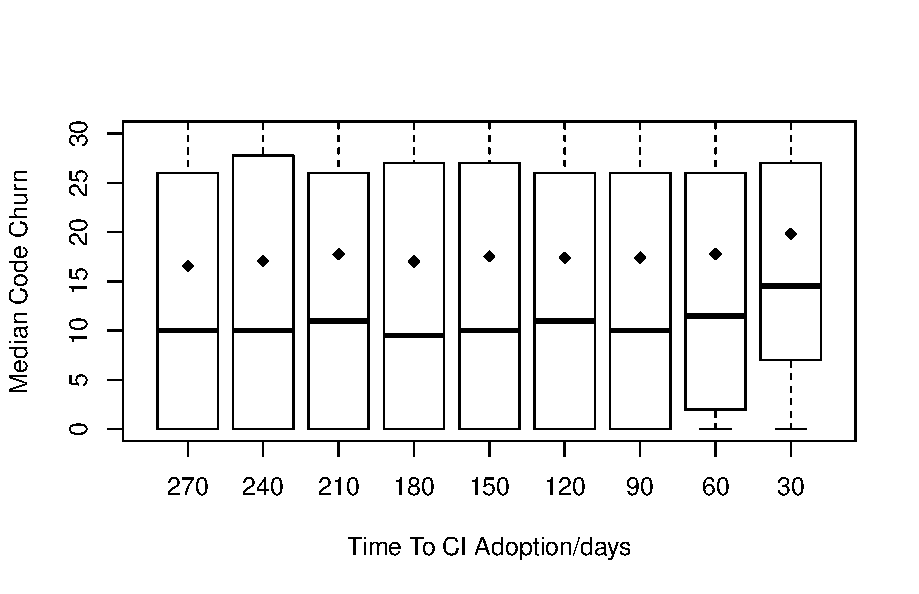
\includegraphics[width=0.45\textwidth, clip=true, trim=0 15 15 50]{churn_before.pdf}
%\caption{Code churn before \Tvis adoption.}
%\label{Fig:CodeChurnBefore}\vspace{-0.3cm}
%\end{figure}
%
%
%\begin{figure}[t]
%\centering
%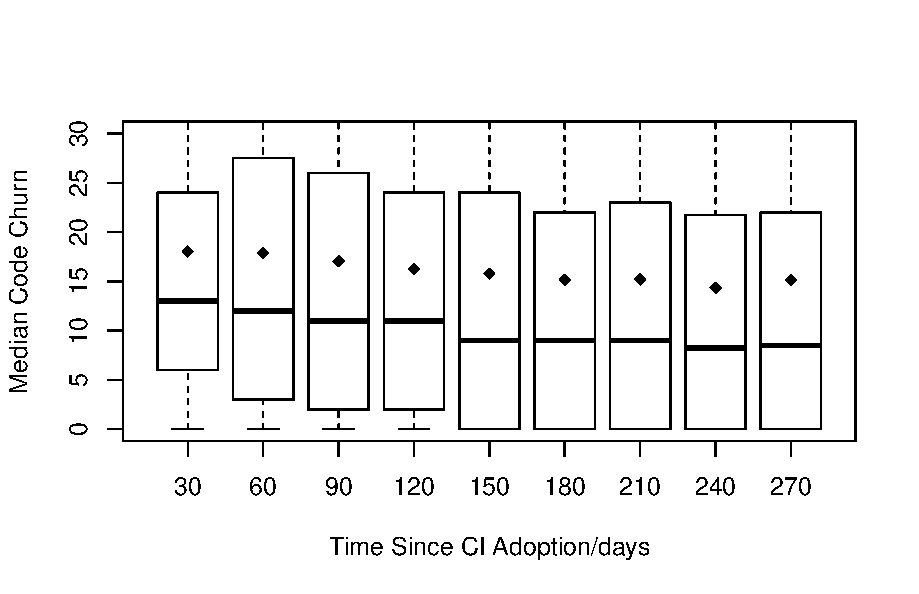
\includegraphics[width=0.45\textwidth, clip=true, trim=0 15 15 50]{churn_after.pdf}
%\caption{Code churn after \Tvis adoption.}
%\label{Fig:CodeChurnAfter}\vspace{-0.3cm}
%\end{figure}



%\as{Vladimir, do you have a cross-combination data, such as \# decrease in churn AND increase in frequency?}

\subsection{RQ3: Trends in Pull Request Closing}

\begin{figure}[t]
\centering
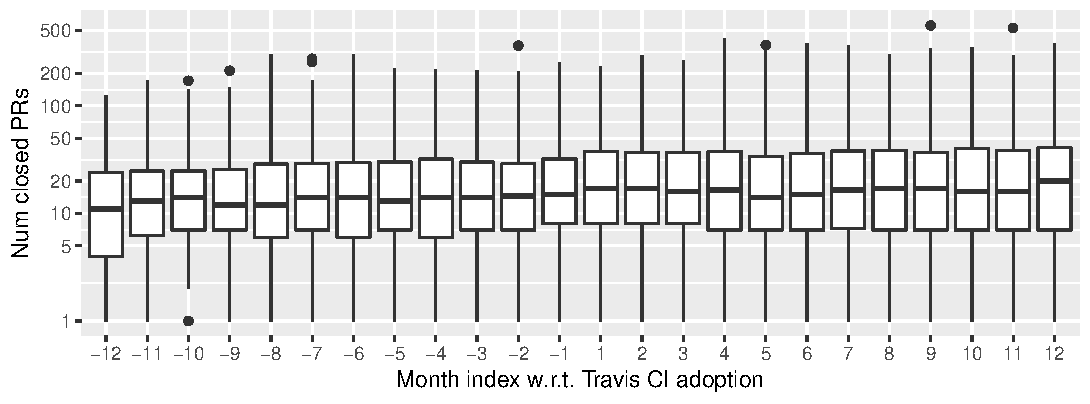
\includegraphics[width=\columnwidth, clip=true, trim=0 0 0 0]{figures/pr-closed.pdf}
\caption{Closed pull requests before and after the \Tvis adoption.}
\label{fig:prs}
\end{figure}


 

\begin{table}[t]
\caption{Pull request model. The response is \textbf{log(number of pull requests closed)}
per month. $R^2_m = 0.32$. $R^2_c = 0.65$.}
\label{table:prs}
 \centering \scriptsize
\rowcolors{3}{Gray}{}
\begin{tabular}{l D{)}{)}{13)3}@{} D{.}{.}{5.5} }
\hline
                                               & \multicolumn{1}{c}{Coeffs (Errors)} & \multicolumn{1}{c}{Sum Sq.} \\
\hline
(Intercept)                            & -3.132 \; (0.356)^{***} & \\
log(TotalCommits)                      & 0.605 \; (0.049)^{***} & 71.17^{***}  \\
AgeAtTravis                            & -0.008 \; (0.001)^{***} & 14.17^{***} \\
log(NumAuthors)                        & 0.136 \; (0.043)^{**}  & 4.64^{**} \\
time                                   & 0.032 \; (0.004)^{***} & 32.98^{***} \\
interventionTRUE                       & 0.005 \; (0.055)       & 0.00 \\
time\_after\_intervention              & -0.033 \; (0.005)^{***} & 18.06^{***} \\
%\hline
%Analysis of Variance Table of type III  with  Satterthwaite 
%approximation for degrees of freedom
%                        Sum Sq Mean Sq NumDF  DenDF F.value    Pr(>F)    
%log(TotalCommits)       71.171  71.171     1  230.0 152.086 < 2.2e-16 ***
%AgeAtTravis             14.169  14.169     1  230.0  30.277 9.956e-08 ***
%log(NumAuthors)          4.640   4.640     1  230.0   9.915  0.001857 ** 
%time                    32.978  32.978     1 5060.0  70.470 < 2.2e-16 ***
%intervention             0.004   0.004     1  622.9   0.009  0.926001    
%time_after_intervention 18.061  18.061     1 5060.0  38.595 5.634e-10 ***

%AIC                                    & 12565.979               \\
%BIC                                    & 12645.373               \\
%Log Likelihood                         & -6270.990               \\
%Num. obs.                              & 5520                    \\
%Num. groups: Repo                      & 230                     \\
%Num. groups: Language                  & 7                       \\
%Var: Repo (Intercept)                  & 0.457                   \\
%Var: Repo interventionTRUE             & 0.340                   \\
%Cov: Repo (Intercept) interventionTRUE & -0.182                  \\
%Var: Language (Intercept)              & 0.000                   \\
%Var: Residual                          & 0.468                   \\
\hline
\rowcolor{white}
\multicolumn{2}{l}{\scriptsize{$^{***}p<0.001$, $^{**}p<0.01$, $^*p<0.05$}}
\end{tabular}\vspace{-0.3cm}
\end{table}




\begin{figure}[t]
\centering
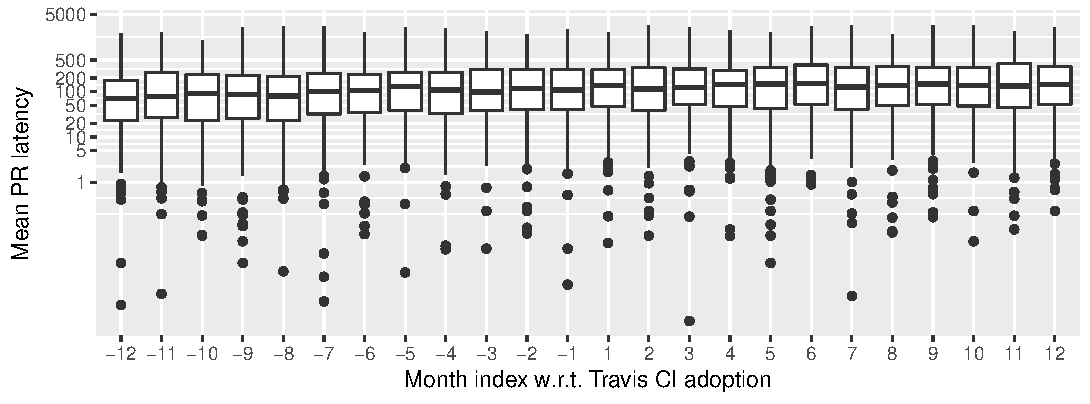
\includegraphics[width=\columnwidth, clip=true, trim=0 0 0 0]{figures/pr-latency.pdf}
\caption{Mean pull request latency before and after the \Tvis adoption.}
\label{fig:pr-latency}
\end{figure}


 

\begin{table}[t]
\caption{Pull request latency model. The response is \textbf{log(mean pull request latency)}
per month, in hours. $R^2_m = 0.05$. $R^2_c = 0.31$.}
\label{table:latency}
\centering \footnotesize
\rowcolors{3}{Gray}{}
\begin{tabular}{l D{)}{)}{13)3}@{} D{.}{.}{5.5} }
\hline
                                               & \multicolumn{1}{c}{Coeffs (Errors)} & \multicolumn{1}{c}{Sum Sq.} \\
\hline
(Intercept)                            & 0.052 \; (0.519)      & \\
log(TotalCommits)                      & 0.157 \; (0.068)^{*} & 7.89^{*}   \\
AgeAtTravis                            & -0.002 \; (0.002)    & 1.00  \\
log(NumAuthors)                        & 0.225 \; (0.062)^{***} & 19.72^{***}\\
time                                   & 0.030 \; (0.012)^{*}  & 8.60^{*} \\
interventionTRUE                       & -0.160 \; (0.153)    & 1.65  \\
time\_after\_intervention              & -0.022 \; (0.019)    & 2.03  \\
\hline
%Analysis of Variance Table of type III  with  Satterthwaite 
%approximation for degrees of freedom
%                         Sum Sq Mean Sq NumDF   DenDF F.value    Pr(>F)    
%log(TotalCommits)        7.8943  7.8943     1  200.00  5.2679 0.0227593 *  
%AgeAtTravis              1.0013  1.0013     1  194.21  0.6682 0.4146849    
%log(NumAuthors)         19.7179 19.7179     1  197.77 13.1579 0.0003644 ***
%time                     8.6001  8.6001     1 1475.42  5.7389 0.0167173 *  
%intervention             1.6486  1.6486     1  886.22  1.1001 0.2945248    
%time_after_intervention  2.0330  2.0330     1 1506.63  1.3566 0.2443056    

%AIC                                    & 5558.908               \\
%BIC                                    & 5623.561               \\
%Log Likelihood                         & -2767.454              \\
%Num. obs.                              & 1616                   \\
%Num. groups: Repo                      & 203                    \\
%Num. groups: Language                  & 7                      \\
%Var: Repo (Intercept)                  & 0.638                  \\
%Var: Repo interventionTRUE             & 0.478                  \\
%Cov: Repo (Intercept) interventionTRUE & -0.342                 \\
%Var: Language (Intercept)              & 0.000                  \\
%Var: Residual                          & 1.499                  \\
%
%(Intercept)                            & 2.510 \; (0.526)^{***} & \\
%log(TotalCommits)                      & -0.138 \; (0.073)    & 6.79 \\
%AgeAtTravis                            & 0.007 \; (0.002)^{***} &  24.44^{***} \\
%log(NumAuthors)                        & 0.474 \; (0.064)^{***} &  101.27^{***} \\
%time                                   & 0.055 \; (0.007)^{***} &  113.44^{***} \\
%interventionTRUE                       & -0.103 \; (0.082)     &  2.95 \\
%time\_after\_intervention              & -0.032 \; (0.010)^{**} &  19.09^{**} \\
%\hline
%AIC                                    & 23087.126              \\
%BIC                                    & 23168.260              \\
%Log Likelihood                         & -11531.563             \\
%Num. obs.                              & 6382                   \\
%Num. groups: Repo                      & 306                    \\
%Num. groups: Language                  & 21                     \\
%Var: Repo (Intercept)                  & 1.085                  \\
%Var: Repo interventionTRUE             & 0.392                  \\
%Cov: Repo (Intercept) interventionTRUE & -0.275                 \\
%Var: Language (Intercept)              & 0.058                  \\
%Var: Residual                          & 1.870                  \\
\hline
\rowcolor{white}
\multicolumn{2}{l}{\scriptsize{$^{***}p<0.001$, $^{**}p<0.01$, $^*p<0.05$}}
\end{tabular} \vspace{-0.4cm}
\end{table}



The next practice we consider is pull request closing, which we analyze along two 
dimensions: the number of pull requests closed, and the average
pull request latency (\ie time to close) per time window.
Since \Tvis is invoked and runs automatically every time a pull request is submitted, 
we expect that developers are rapidly notified whether their pull request passes the 
\Tvi-quality gate.
This would mean that they can rapidly react to the feedback provided by \Tvi and 
correct the pull request source code if necessary.
Overall, we therefore expect that \Tvis should shorten the pull request latency and, 
under the assumption of constant productivity, increase the number of pull requests 
being closed.
\as{some literature here. Bogdan, is ``Wait for it'' relevant here?}

\smallskip\noindent \emph{Exploratory Study}:
Figure
%s~\ref{fig:issues} and 
\ref{fig:prs} shows boxplots of per-project number of closed pull requests, for each 
of twelve consecutive 30-day time intervals before, and after, the \Tvis adoption. 
Similarly to Figure~\ref{fig:churn}, in both cases we see large variance around the 
medians. 
Inspecting the figure we observe that the median number of closed pull requests 
per months fluctuates between 11 and 15 across the twelve periods pre-\Tvi, and 
between 14 and 20 across the twelve periods post adoption.
We note an apparent increasing trend pre-\Tvi, which also seems to continue post-\Tvi.
%seems to fluctuate around 12 \as{can we take a look at the numbers?}
%and while the number of closed issues does not seem to exhibit any trend, the number of closed pull requests seems to be increasing after the introduction of \Tvis.

Figure~\ref{fig:pr-latency} provides a complementary perspective on the efficiency 
of pull request resolution, namely the pull request latency.
The median latency seems to increase prior to introduction of \Tvis, and continues
to do so afterwards. % and more or less to stabilize after \Tvis has been introduced.

\smallskip\noindent \emph{Statistical Modeling Study}:
We apply RDD as above. 
%in the same way we have using this approach to address \textbf{RQ1} and \textbf{RQ2}. 
The statistical models for the number of pull requests closed and the mean pull 
request latency are summarized in Tables~\ref{table:prs} and \ref{table:latency}.
As above, the combined fixed-and-random effects models fit the data much 
better than the basic fixed-effect models, indicating that the project-to-project 
and language-to-language variability are responsible for most of the variability 
explained.
%$R^2_m$ and $R^2_c$ are in line with the statistical models built for \textbf{RQ2} 
%(churn), with $R^2_m \simeq 0.1-0.2$ and $R^2_c \simeq 0.4-0.5$.

Regarding closed pull requests (Table~\ref{table:prs}), we note an increasing
\emph{time} baseline trend pre-adoption; no statistically significant discontinuity
at the adoption time; and an apparent neutralization of the aforementioned time
trend post-adoption, as $\beta$(\emph{time}) $+$ 
$\gamma$(\emph{time\_after\_intervention}) $\simeq 0$.

Turning to the pull request latency model (Table~\ref{table:latency}), we note
a statistically significant, increasing baseline \emph{time} trend, which remains
unaffected by the \Tvis adoption, as neither coefficient for discontinuity and
change in trend has statistically significant effects.

%observe that the number of authors is statistically significant and explains a 
%large part of the variance explained by the model.
%Variable \emph{time} is also statistically significant and explains a big percentage of the variance. 
%This means that there is a base-line increase in the pull request latency; introduction of \Tvis does not result in a discontinuity (\emph{intervention} is not statistically significant) but merely slows down the increasing trend.

%Recall, that as opposed to Yu et al.~\cite{yue2015wait} we consider as authors 
%\emph{both} core developers, with commit rights, and external contributors that can only submit pull requests. 
%Our model indicates that projects with larger number of authors tend to have a higher pull
%request latency, suggesting that the larger number of authors is achieved through a high
%number of external contributors submitting pull requests and therefore slowing down the pull request review process as each pull request requires an extra review/merge effort from a limited number of core developers.

\smallskip\noindent \emph{Discussion}:

The statistical modeling study generated two noteworthy findings.
First, despite a visually apparent increasing trend in the number of pull requests 
closed per time period, across the entire interval under observation, our model 
suggests that, after controling for project size, project age, and size of developer 
community, as well as local project-to-project and language-to-language differences, 
the increasing trend manifests itself, in aggregate, only pre-\Tvi.
Moreover, and quite surprisingly, we find that the initial trend is flattened post-\Tvi,
resulting in relatively stationary behavior, on average.
This paints a more nuanced picture of how \GH teams are adapting to, and
benefiting from, continuous integration technology than suggested by prior
work~\cite{VasilescuYWDF15}, and speaks to the strength of time-series-based
analysis methods, such as the RDD we use here, at detecting fine resolution effects.

Second, our model finds that, on average, pull requests are taking longer to close 
over time, and this trend is unaffected by the switch to \Tvis.
This, again, is quite surprising, as we have seen in RQ2 above that the size of 
code changes becomes, on average, smaller and smaller over time; in turn, this
would imply that changes are also easier (quicker) to evaluate.
\as{Talk about survey and how Travis is becoming slow, which may explain latency trend}



\subsection{RQ4: Trends in Issue Closing}

Next, we examine issue closing trends.
%As above, we use data on 293 projects, each with 
%100+ issues.

\begin{figure}[t]
\centering
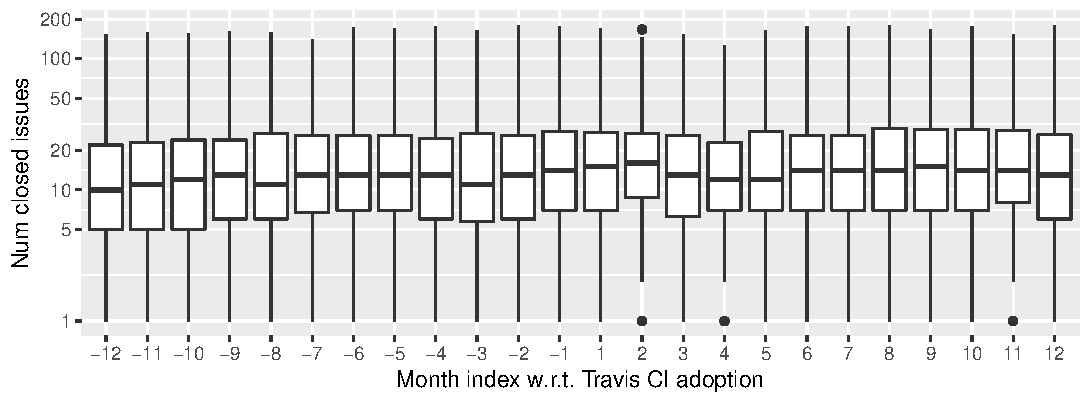
\includegraphics[width=\columnwidth, clip=true, trim=0 0 0 0]{figures/issues-closed.pdf}
\caption{Number of closed issues before and after the \Tvis adoption.}
\label{fig:issues}
\end{figure}



 

\begin{table}[t]
\centering \footnotesize
\rowcolors{3}{Gray}{}
\begin{tabular}{l D{)}{)}{13)3}@{} D{.}{.}{5.5} }
\hline
                                               & \multicolumn{1}{c}{Coeffs (Errors)} & \multicolumn{1}{c}{Sum Sq.} \\
\hline
(Intercept)                            & -1.680 \; (0.364)^{***} & \\
log(TotalCommits)                      & 0.443 \; (0.049)^{***} & 42.54^{***}  \\
AgeAtTravis                            & -0.006 \; (0.001)^{***} & 8.83^{***}\\
log(NumAuthors)                        & 0.119 \; (0.039)^{**}   & 4.72^{**}\\
time                                   & 0.021 \; (0.004)^{***}  & 16.00^{***}\\
interventionTRUE                       & 0.030 \; (0.049)         0.19&\\
time\_after\_intervention              & -0.019 \; (0.005)^{***}  &  5.99^{***}\\
\hline
%AIC                                    & 13679.398               \\
%BIC                                    & 13759.398               \\
%Log Likelihood                         & -6827.699               \\
%Num. obs.                              & 5806                    \\
%Num. groups: Repo                      & 280                     \\
%Num. groups: Language                  & 20                      \\
%Var: Repo (Intercept)                  & 0.403                   \\
%Var: Repo interventionTRUE             & 0.213                   \\
%Cov: Repo (Intercept) interventionTRUE & -0.134                  \\
%Var: Language (Intercept)              & 0.019                   \\
%Var: Residual                          & 0.513                   \\
%
%(Intercept)                            & -2.540 \; (0.180)^{***} & \\
%log(TotalCommits)                      & 0.396 \; (0.025)^{***} & 155.91^{***} \\
%AgeAtTravis                            & -0.006 \; (0.001)^{***} & 47.72^{***}\\
%log(NumAuthors)                        & 0.224 \; (0.019)^{***} & 83.73^{***} \\
%time                                   & 0.012 \; (0.002)^{***} & 13.58^{***} \\
%interventionTRUE                       & 0.049 \; (0.028)       & 2.02 \\
%time\_after\_intervention              & -0.008 \; (0.003)^{*}  & 3.77^{*} \\
%\hline
%AIC                                    & 58524.762               \\
%BIC                                    & 58620.964               \\
%Log Likelihood                         & -29250.381              \\
%Num. obs.                              & 22401                   \\
%Num. groups: Repo                      & 1716                    \\
%Num. groups: Language                  & 22                      \\
%Var: Repo (Intercept)                  & 0.641                   \\
%Var: Repo interventionTRUE             & 0.301                   \\
%Cov: Repo (Intercept) interventionTRUE & -0.159                  \\
%Var: Language (Intercept)              & 0.050                   \\
%Var: Residual                          & 0.627                   \\
\hline
\rowcolor{white}
\multicolumn{2}{l}{\scriptsize{$^{***}p<0.001$, $^{**}p<0.01$, $^*p<0.05$}}
\end{tabular}
\caption{Issues model. The response is \textbf{log(number of issues closed)}
per month. $R^2_m = 0.17$. $R^2_c = 0.53$.}
\label{table:issues}
 
\end{table}





%
%\begin{figure}[t]
%\centering
%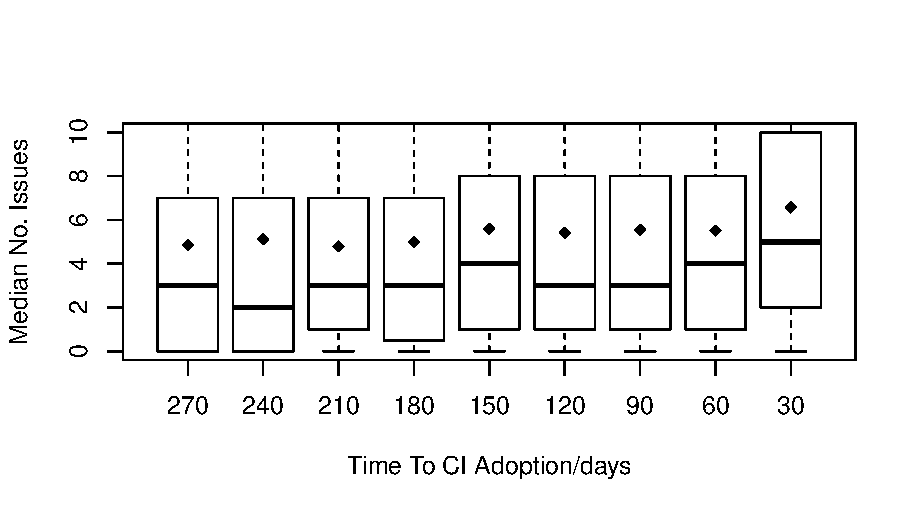
\includegraphics[width=0.45\textwidth, clip=true, trim=0 15 15 50]{issues_before.pdf}
%\caption{Median number of issues before CI adoption}
%\label{Fig:IssuesBefore}
%\end{figure}
%
%
%\begin{figure}[t]
%\centering
%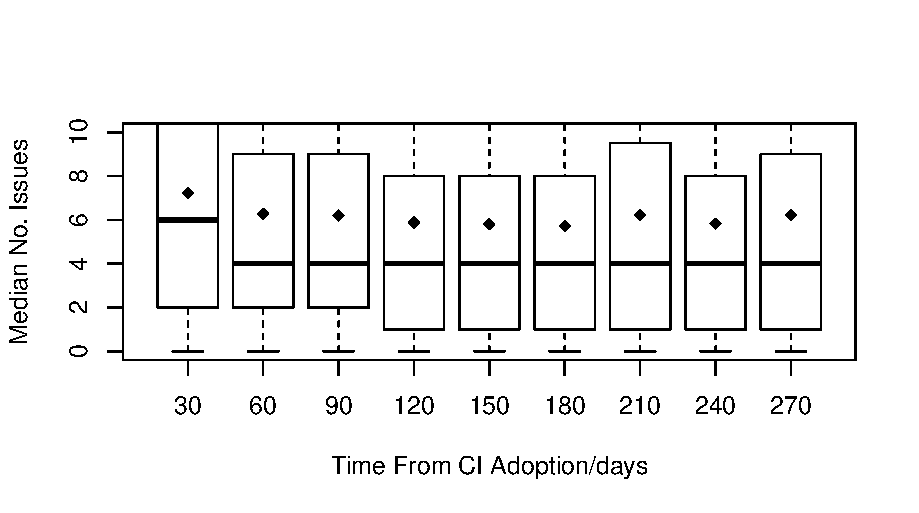
\includegraphics[width=0.45\textwidth, clip=true, trim=0 15 15 50]{issues_after.pdf}
%\caption{Median number of issues after CI adoption}
%\label{Fig:IssuesAfter}
%\end{figure}

\smallskip\noindent \emph{Exploratory Study}:
We follow the same approach as above and compare the 
medians in the number of issues per time period, in the months before and after CI adoption.
Fig.~\ref{fig:issues} shows the boxplots of the number of 
issues per unit time period for 12 consecutive 30-day time intervals, before and after \Tvis adoption.
We note that the month immediately preceding 
and the two following the adoption exhibit the highest number of issues.
Besides those, before CI adoption the median number of issues per period seems to vary between 10 and 13, with most of them being in between.
Following CI adoption, we note a slight increasing trend in the median of the number of issues closed, with the median between 12 and 14.

%% !TEX root = ../CI_Adoption.tex

\begin{table}[t] \centering
\small
  \caption{Model Coefficients for 291 Models of Issues Frequency}
  \label{Table:rddmodels_freq}
\begin{tabular}{ l  r r r r }        
\hline 

 & $\beta$ & $\gamma$ & $\delta$ & $\beta + \delta$ \\ 
 \hline 
 \hline
not signif. & 230 & 254 & 242 & \\
\hline
signif., $>0$ & 43 & 26 & 14 & 15 \\
\hline
signif., $<0$ & 18 & 11 & 35 & 33 \\
\hline
\end{tabular}
\end{table}

\smallskip\noindent \emph{Statistical Modeling Study}:
We apply RDD as above. 
%in the same way we have using this approach to address \textbf{RQ1} and \textbf{RQ2}. 
The statistical model for the number of issues closed is summarized in Table~\ref{table:issues}.
As above, the combined fixed-and-random effects models fit the data much 
better than the basic fixed-effect models, indicating that the project-to-project 
and language-to-language variability are responsible for most of the variability 
explained.
%$R^2_m$ and $R^2_c$ are in line with the statistical models built for \textbf{RQ2} 
%(churn), with $R^2_m \simeq 0.1-0.2$ and $R^2_c \simeq 0.4-0.5$.
We note an increasing
\emph{time} baseline trend pre-adoption; no statistically significant discontinuity
at the adoption time; and a slight positive trend post-adoption, as $\beta$(\emph{time}) $+$ 
$\gamma$(\emph{time\_after\_intervention}) $> 0$.


%Results of the RDD modeling are summarized in Table~\ref{Table:rddmodels_issues}.
%The time period before and the one after the time of CI adoption have been removed from the modeling, as explained in RQ1 above.
%The lower number of projects in Table~\ref{Table:rddmodels_issues} 
%compared to Tables~\ref{Table:rddmodels} and~\ref{Table:rddmodels_freq} 
%should not be surprising. 
%Recall from Section~\ref{sec:dd} that to answer RQ3 we have focused on 
%projects having at least 100 issues, further reducing the size of the data set 
%used in RQ1 and RQ2 to 293.
%We have fitted models to 291 projects of the 293, however in most cases we 
%did not observe linear trends.
%When a linear trend has been observed than it was more than twice more 
%often decreasing than increasing.
%The mean value over all projects for $\gamma$, the effect size of CI adoption, 
%was $1.0$ issue.


\smallskip\noindent \emph{Discussion}:
%Again, most of the projects did not have longitudinal linear trends for reasons probably similar to those in the case of the code churn.
%
%As in RQ1, our exploratory study showed a peak in the median number of issues per period around CI adoption time, and an upward trend following CI adoption.
%The modeling study showed that when linear trends were present (in 20\% 
%of the models), the downward one after CI adoption were 2.5 times as frequent 
%as the upward one, a reversal of the pattern in the trends from before CI.
%This has to be considered in combination with the size of the effect of CI adoption, which is $1$ issue per period additional.
%Thus, the number of issues increases significantly overall after CI adoption, to the tune of $33\%$, and then has a pressure of slight reduction over time.
The statistical modeling study confirmed the visually apparent increasing trend in the number of issues 
closed per time period, across the entire interval under observation, although the trend slows down following \Tvis adoption, and is smaller than expected from the visual study, indicating the moderating influence of the control variables.
Thus, our model finds that, on average, more issues are being closed 
over time, but this trend slows with the switch to \Tvis.






\as{Survey}
Survey participants experience \Tvi as beneficial for bug detection: ``I think we produce less bugs'' (R45), ``there was an immediately noticeable improvement in terms of the number of serious bugs in production'' (R51). 
An interesting insight into this matter is provided by R16: while several survey respondents have indicated that \Tvis is not consistent in terms of performance and relatively slow, those performance aspects provided R16 with means to detect ``more flaky issues'' ``which where only visible on \Tvi''. 

\subsection{RQ5: Trends in Testing}

The last development practice we examine is testing.
% and the evolution 
%of the types of errors revealed by automated testing.
Here we only consider a sample of Java projects, for which we could confidently
identify their build system and, consequently, parse their \Tvi log files. 
The sample consists of 250 projects, each with at least 100 builds, 90+\% of 
builds executing tests.

\begin{figure}[!t]
\centering
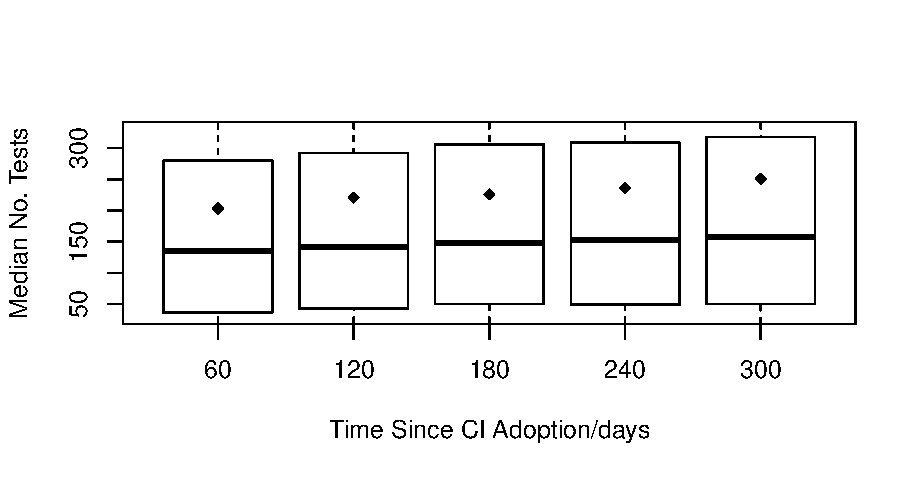
\includegraphics[width=0.4\textwidth, clip=true, trim=0 15 15 50]{tests.pdf}
\caption{Unit tests per build following CI adoption.}\vspace{-0.3cm}
\label{Fig:Tests}
\end{figure}

\smallskip\noindent \emph{Exploratory Study}: 
As before, we first look for general trends.
Fig.~\ref{Fig:Tests} shows a boxplot of per-project median number of tests 
per build, for each of five consecutive 60-day time intervals before CI adoption.
We aggregated the data here in 60 day intervals to make it easier to visualize 
the trend, since the differences are small.
The horizontal line in each boxplot is the median value of all per-project medians, 
and the black dot is their average value.
We observe a monotonically increasing trend in both the medians, from 140 to 
160 tests per build, and the means, from 205 to 245, \ie 15\% to 20\% increase. 

To ascertain if the complexity of builds increases over time, we also calculated 
the average number of jobs per build.
The median is $1$ for all five time intervals.
These two findings suggest strongly that there is an increase in the number of 
unit tests per build over time.
This, coupled with our finding that builds are not getting more complex over time 
indicates that developers are likely spending more time on automated testing 
since CI adoption.
This is consistent with Fowler's ``good practices" proposal.

\smallskip\noindent \emph{Error Types Study}:
We also looked at the evolution of the error types in builds over time after CI 
adoption.
For all 250 projects above, we looked at the builds that resulted in errors, 
and deconvolved the errors into 8 types after open coding.
We did this over 3 intervals: 0-60 days, 61-180 days, and 181-300 days (\ie 
corresponding to the first, third, and fifth interval in Figure~\ref{Fig:Tests}).
%The results are shown in Figure~\ref{Fig:BugTypes}, where on the $y$-axis are 
%the proportion of all erroneous builds that yield that error type.
We find an apparent upward trend over time in most error type categories, 
most notably compile errors, execution errors, failed tests, and skipped 
test.\footnote{The median number of error types per build remained $2$ over 
time.}
All these are consistent with an increase in the amount of code being built 
and tested per build, as well as an increasing management of errors by 
skipping tests, likely to aid in debugging.
On the other hand, we find a decreasing trend among errors related to missing 
files/dependencies, and time-outs, both consistent with those errors being less 
of an issue over time, as developers are acculturating to the CI mediated 
processes.

Thus, overall we find an expected adjustment to the automated testing and 
error handling, with an indication that debugging complexity grows over time.

%%this is the old plots
%\begin{figure}[!t]
%\centering
%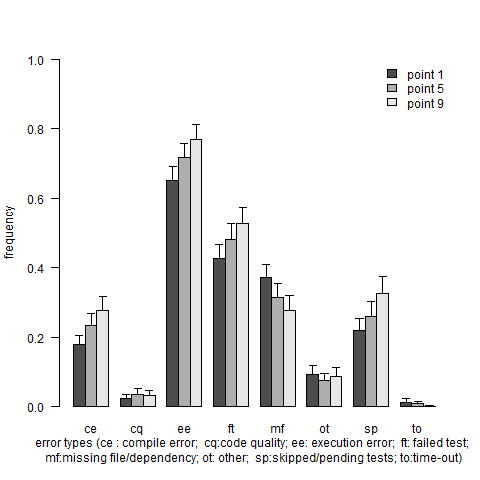
\includegraphics[width=0.45\textwidth, clip=true, trim=0 15 15 50]{plot_together.png}
%\caption{Evolution of Error Types Since CI Adoption}
%\label{Fig:BugTypesold}
%\end{figure}


%this is the new plots
%\begin{figure}[!t]
%	\centering
%	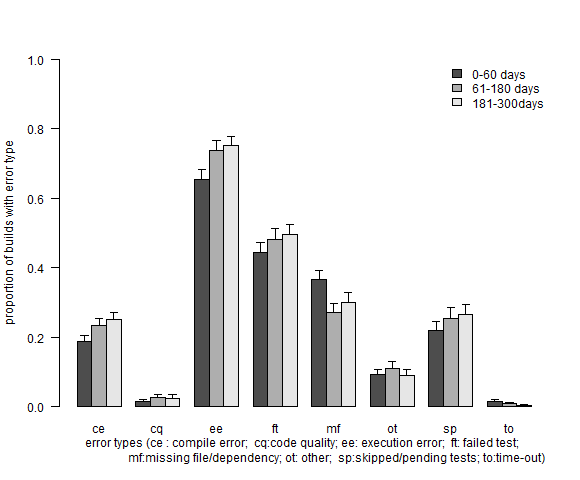
\includegraphics[width=0.45\textwidth, clip=true, trim=0 15 15 50]{new_plot_together.png}
%	\caption{Evolution of Error Types Since CI Adoption}
%	\label{Fig:BugTypes}
%\end{figure}

\as{Survey}
Improving software quality through test automation has been repeatedly mentioned 
by the survey respondents as a reason to switch to \Tvis. 
Not surprisingly, respondents also indicate that changes facilitating test automation 
had to be made when \Tvis was introduced. 
Moreover, by using \Tvis developers became more aware of testing-related aspects 
of their software development process (R32, R52), spent more time and effort on 
designing testing strategies (R5, R53), and encouraged other projects to start using 
\Tvis (R26).
The efficiency of \Tvis for long-running tests is, however, a concern (R10).

